\chapter{API Contract and Integration Design}

\section{What is an API and Why Does Lucid Use One?}
To understand how Lucid's website communicates with its calculation engine, it helps to use the analogy of a restaurant:
\begin{itemize}
    \item \textbf{The Customer (The User Interface / Frontend)}: The investor interacts with buttons, forms, and charts displayed in their web browser (built with Next.js and React).
    \item \textbf{The Kitchen (The Backend Server and Database)}: The backend server runs the 13 AI agents, accesses 2,639 listed Indian companies, and executes mathematical solvers to optimize portfolios.
    \item \textbf{The Waiter (The API)}: An \textbf{Application Programming Interface (API)} acts as the professional waiter. When the investor clicks ``Generate Portfolio,'' the waiter takes the customer's order to the kitchen, ensures the kitchen prepares it according to the customer's rules, and brings the final dish (the recommended portfolio) back to the table in a clean, organized format.
\end{itemize}

Because Lucid's frontend and backend are decoupled, the website never touches the database directly. Every interaction occurs through secure, standardized API messages.

\section{Core Rules of Lucid's API Communication}
Lucid follows four foundational design principles to ensure fast, secure, and reliable communication:
\begin{enumerate}
    \item \textbf{Standardized Base URL and Versioning}: All API routes begin with the prefix \texttt{/api/v1/}. Versioning ensures that if new features are added in the future (such as \texttt{/api/v2/}), existing apps continue working without breaking.
    \item \textbf{Secure Digital Session Badges (JWT Tokens)}: When a user logs in, the server gives them a temporary, cryptographically signed digital pass (called a \textbf{JSON Web Token} or JWT). For every subsequent action (such as saving a goal or checking holdings), the browser presents this badge in the request header (\texttt{Authorization: Bearer <token>}). This proves the user's identity without requiring them to re-enter their password for every click. Tokens expire after 60 minutes for safety.
    \item \textbf{Strict Input Inspection (Pydantic v2)}: The server inspects every incoming message before processing it. If a user tries to enter negative money, an invalid email address, or an unrecognized stock ticker, the server immediately stops the request and returns a friendly error message, protecting the system from bad data.
    \item \textbf{Predictable Status Codes}: Lucid uses standard international web response codes:
    \begin{itemize}
        \item \texttt{200 OK}: The request was successful, and the requested information is returned.
        \item \texttt{201 Created}: A new record (such as a newly generated portfolio or saved financial goal) was created successfully.
        \item \texttt{400 Bad Request}: The request contained invalid information (such as entering an investment amount below the minimum Rs.~5,000 threshold).
        \item \texttt{401 Unauthorized}: The user has not logged in or their session token has expired.
        \item \texttt{429 Too Many Requests}: The user is sending requests too quickly, activating rate-limiting protections.
        \item \texttt{500 Internal Server Error}: An unexpected technical error occurred on the server.
    \end{itemize}
\end{enumerate}

\section{Complete API Inventory: 82 Active Endpoints}
The Lucid backend provides exactly \textbf{82 unique API endpoints} organized into eleven functional groups, as detailed in Table~\ref{tab:api_domain_inventory}:

\begin{table}[H]
\centering
\caption{Lucid Complete API Endpoint Domain Inventory (82 Endpoints)}
\label{tab:api_domain_inventory}
\resizebox{\textwidth}{!}{%
\begin{tabular}{lcl}
\toprule
\textbf{Functional API Domain} & \textbf{Routes} & \textbf{Primary Routes and Key Operations} \\
\midrule
\textbf{1. Authentication \& Security} & 8 & \texttt{/auth/login}, \texttt{/auth/register}, \texttt{/auth/logout}, \texttt{/auth/me}, \texttt{/auth/change-password} \\
\textbf{2. User Profile \& Preferences} & 6 & \texttt{/profile}, \texttt{/profile/preferences}, \texttt{/profile/security-preferences}, \texttt{/profile/sector-preferences} \\
\textbf{3. Financial Goal Management} & 5 & \texttt{/goals}, \texttt{/goals/\{id\}}, \texttt{/goals/\{id\}/progress}, \texttt{/goals/\{id\}/link-portfolio} \\
\textbf{4. Risk Questionnaire \& Scoring} & 5 & \texttt{/risk-questions}, \texttt{/risk-questions/\{id\}}, \texttt{/risk-assessments}, \texttt{/risk-assessments/latest} \\
\textbf{5. Security Master \& Search} & 10 & \texttt{/securities}, \texttt{/securities/search}, \texttt{/securities/\{isin\}}, \texttt{/securities/sectors}, \texttt{/securities/tickers} \\
\textbf{6. Market Data, Prices \& Regime} & 8 & \texttt{/market-data/prices/\{symbol\}}, \texttt{/market-data/regime}, \texttt{/market-data/indicators} \\
\textbf{7. Portfolio Engine \& Generation} & 12 & \texttt{/portfolio-generation-requests}, \texttt{/portfolios}, \texttt{/portfolios/\{id\}/versions/\{v\}/stocks/\{sym\}/why} \\
\textbf{8. Demat Statement Diagnosis} & 6 & \texttt{/diagnosis/upload-cas}, \texttt{/diagnosis/analyze/\{id\}}, \texttt{/diagnosis/\{id\}/chat}, \texttt{/diagnosis/\{id\}/holdings} \\
\textbf{9. Continuous Monitoring \& Drift} & 6 & \texttt{/monitoring/\{portfolio\_id\}}, \texttt{/monitoring/\{id\}/drift}, \texttt{/monitoring/scheduler/status} \\
\textbf{10. Rebalancing \& Orders} & 8 & \texttt{/rebalancing/evaluate/\{id\}}, \texttt{/rebalancing/preview/\{id\}}, \texttt{/rebalancing/orders/generate} \\
\textbf{11. Notifications \& System Health} & 8 & \texttt{/notifications}, \texttt{/notifications/unread-count}, \texttt{/notifications/\{id\}/read}, \texttt{/api/health} \\
\bottomrule
\textbf{Total Active API Routes} & \textbf{82} & \textbf{100\% Verified and Documented via OpenAPI Specification} \\
\bottomrule
\end{tabular}%
}
\end{table}

\section{Detailed Walkthrough of Core API Interactions}

\subsection{1. Generating a New Investment Portfolio}
When an investor completes the onboarding flow and requests a portfolio, the browser sends a \texttt{POST} request to \texttt{/api/v1/portfolio-generation-requests}:

\noindent \textbf{The Request (What the Browser Sends)}:
\begin{footnotesize}
\begin{verbatim}
{
  "investment_amount": 250000.0,
  "risk_category": "moderate",
  "goal_id": "3fa85f64-5717-4562-b3fc-2c963f66afa6",
  "time_horizon_years": 10,
  "excluded_sectors": ["FMCG_TOBACCO"]
}
\end{verbatim}
\end{footnotesize}

\noindent \textbf{The Response (What the Server Delivers Back)}:
The server coordinates the 13 AI agents, runs the SciPy SLSQP optimizer, rounds shares to whole integer counts, and returns a complete, executable portfolio in approximately 2.1 seconds:
\begin{footnotesize}
\begin{verbatim}
{
  "portfolio_id": "c1f7b8a2-8924-4b5a-9311-c9182046ef12",
  "version_number": 1,
  "total_invested_amount": 248920.0,
  "cash_balance": 1080.0,
  "allocated_stocks_count": 12,
  "expected_annual_return_pct": 14.8,
  "annualized_volatility_pct": 11.2,
  "sharpe_ratio": 0.70,
  "holdings": [
    {
      "symbol": "TCS",
      "company_name": "Tata Consultancy Services Ltd.",
      "sector": "Information Technology",
      "allocated_shares": 18,
      "buy_price": 3850.0,
      "allocated_amount": 69300.0,
      "target_weight_pct": 24.5
    }
  ]
}
\end{verbatim}
\end{footnotesize}

\subsection{2. Asking ``Why Was This Stock Chosen?'' (Stock-Why API)}
When a user clicks on an individual company in their portfolio to understand why it was selected, the browser sends a \texttt{GET} request to the Stock-Why endpoint (\path{/api/v1/portfolios/{id}/versions/{v}/stocks/{symbol}/why}):

\noindent \textbf{The Response Delivered to the User}:
\begin{footnotesize}
\begin{verbatim}
{
  "symbol": "TCS",
  "company_name": "Tata Consultancy Services Ltd.",
  "allocated_weight_pct": 24.5,
  "retail_narrative": "TCS was selected for its 46% ROE, "
                     "near-zero debt, and high cash flow.",
  "factor_metrics": {
    "pe_ratio": 28.4,
    "roe_pct": 46.2,
    "debt_to_equity": 0.08,
    "marginal_risk_contribution_pct": 18.2
  }
}
\end{verbatim}
\end{footnotesize}

\subsection{3. Uploading and Diagnosing a Demat Account Statement}
When an investor uploads their monthly Demat statement (PDF format), the browser sends a \path{multipart/form-data} request to the CAS diagnosis endpoint (\path{/api/v1/diagnosis/upload-cas}). The server parses the document and responds with a complete health diagnostic:
\begin{footnotesize}
\begin{verbatim}
{
  "diagnosis_id": "d9812401-291b-419a-9e12-b21908239014",
  "total_holdings_count": 8,
  "total_valuation": 412500.0,
  "hhi_score": 2840.0,
  "concentration_risk": "HIGH",
  "overlapping_stocks": ["RELIANCE", "INFY"],
  "recommendation_summary": "Portfolio concentrated in two large-caps. "
                            "Adding mid-caps is recommended."
}
\end{verbatim}
\end{footnotesize}

\section{API Sequence Interaction Flows}
Figures~\ref{fig:api_auth_seq} through \ref{fig:api_diag_seq} display the step-by-step sequence diagrams for the primary user workflows:

\clearpage
\begin{figure}[p]
    \centering
    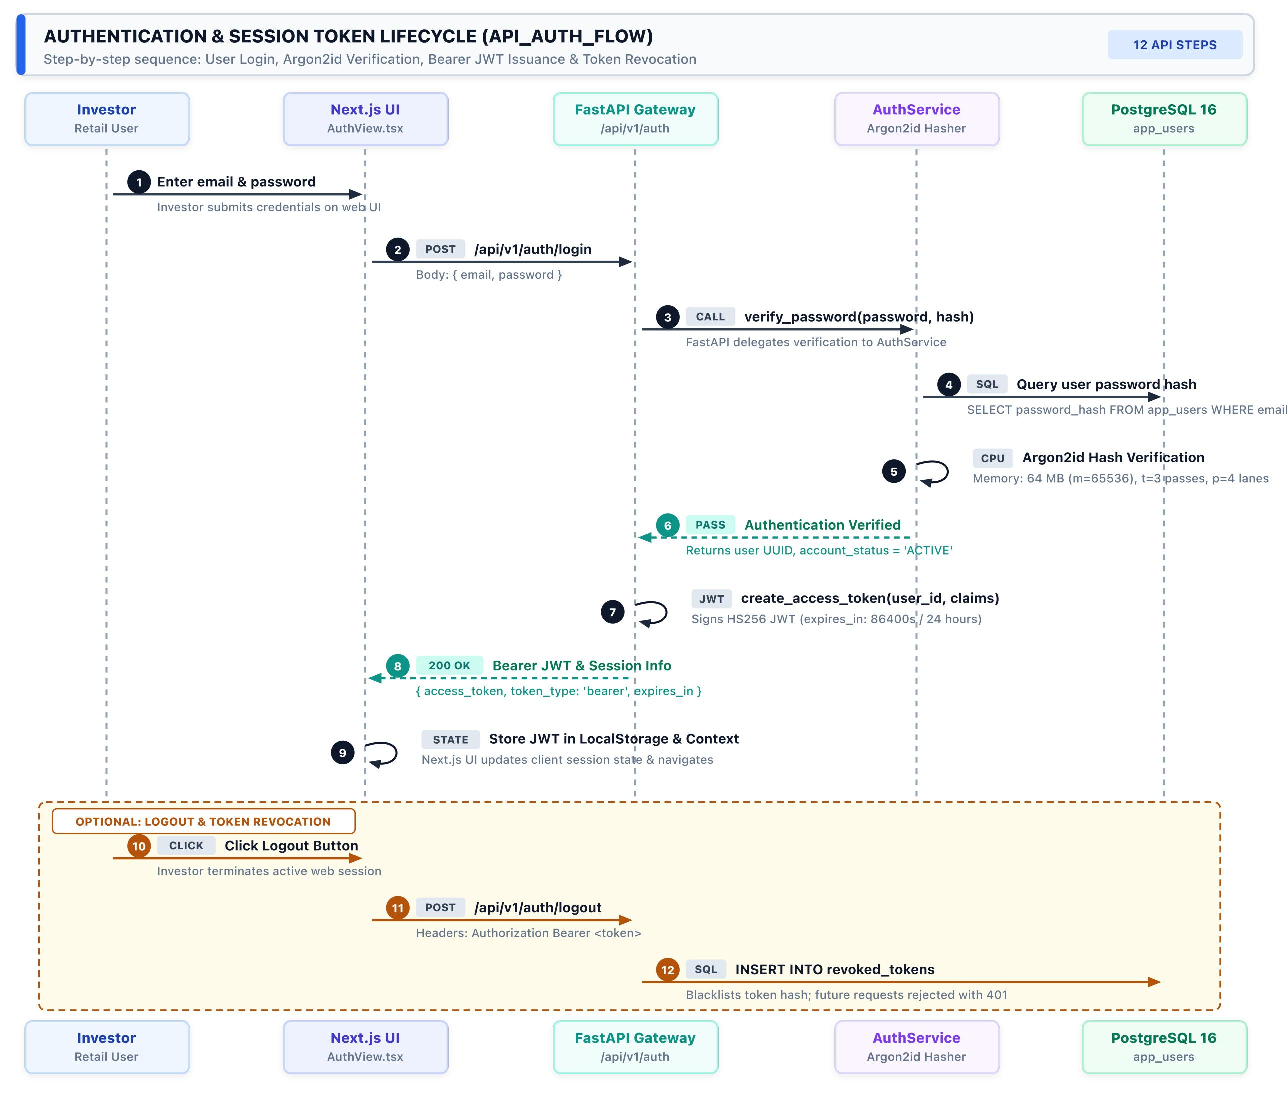
\includegraphics[width=\textwidth, height=0.72\textheight, keepaspectratio]{API_AUTH_FLOW.pdf}
    \caption{API Sequence Diagram: User Registration, Login, and Session Token Flow}
    \label{fig:api_auth_seq}
\end{figure}

\clearpage
\begin{figure}[p]
    \centering
    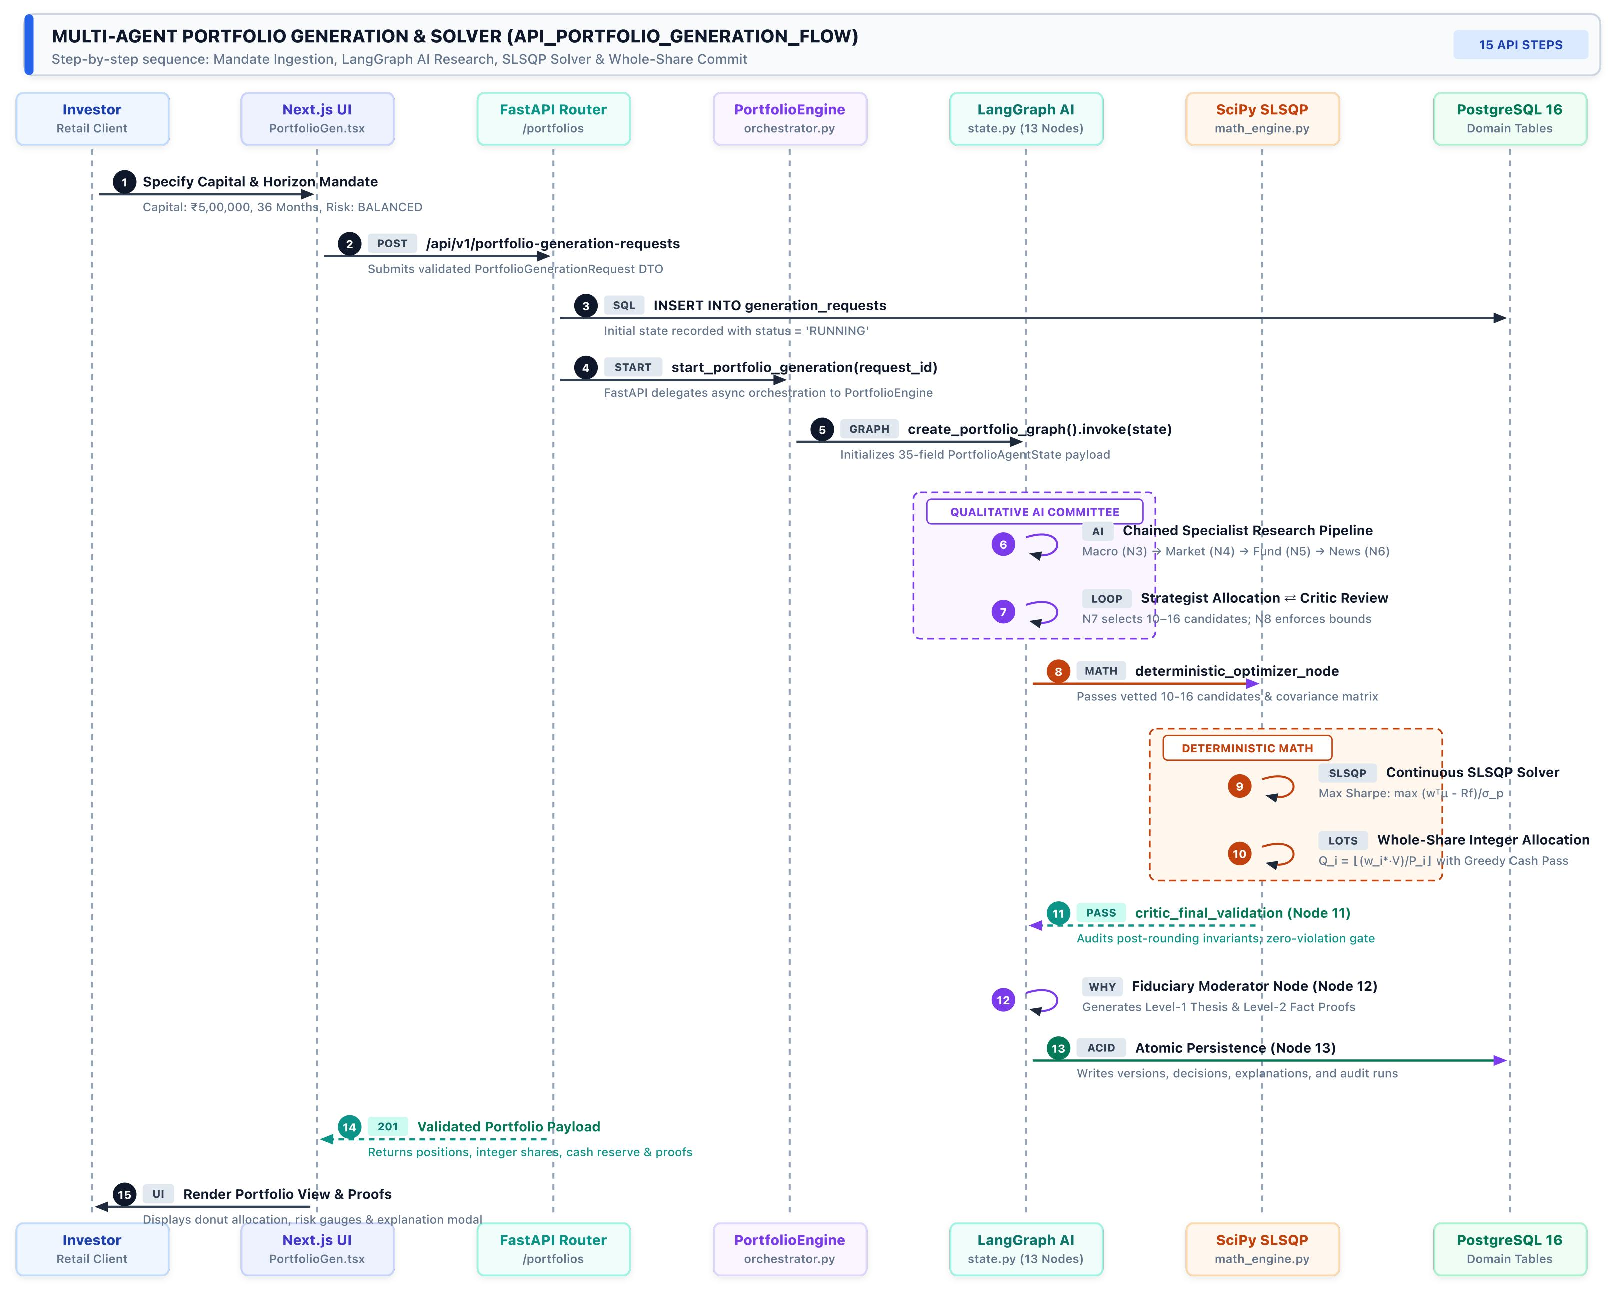
\includegraphics[width=\textwidth, height=0.72\textheight, keepaspectratio]{API_PORTFOLIO_GENERATION_FLOW.pdf}
    \caption[API Sequence Diagram: Multi-Agent Portfolio Solver Flow]{API Sequence Diagram: Multi-Agent Portfolio Generation and Solver Flow}
    \label{fig:api_port_seq}
\end{figure}

\clearpage
\begin{figure}[p]
    \centering
    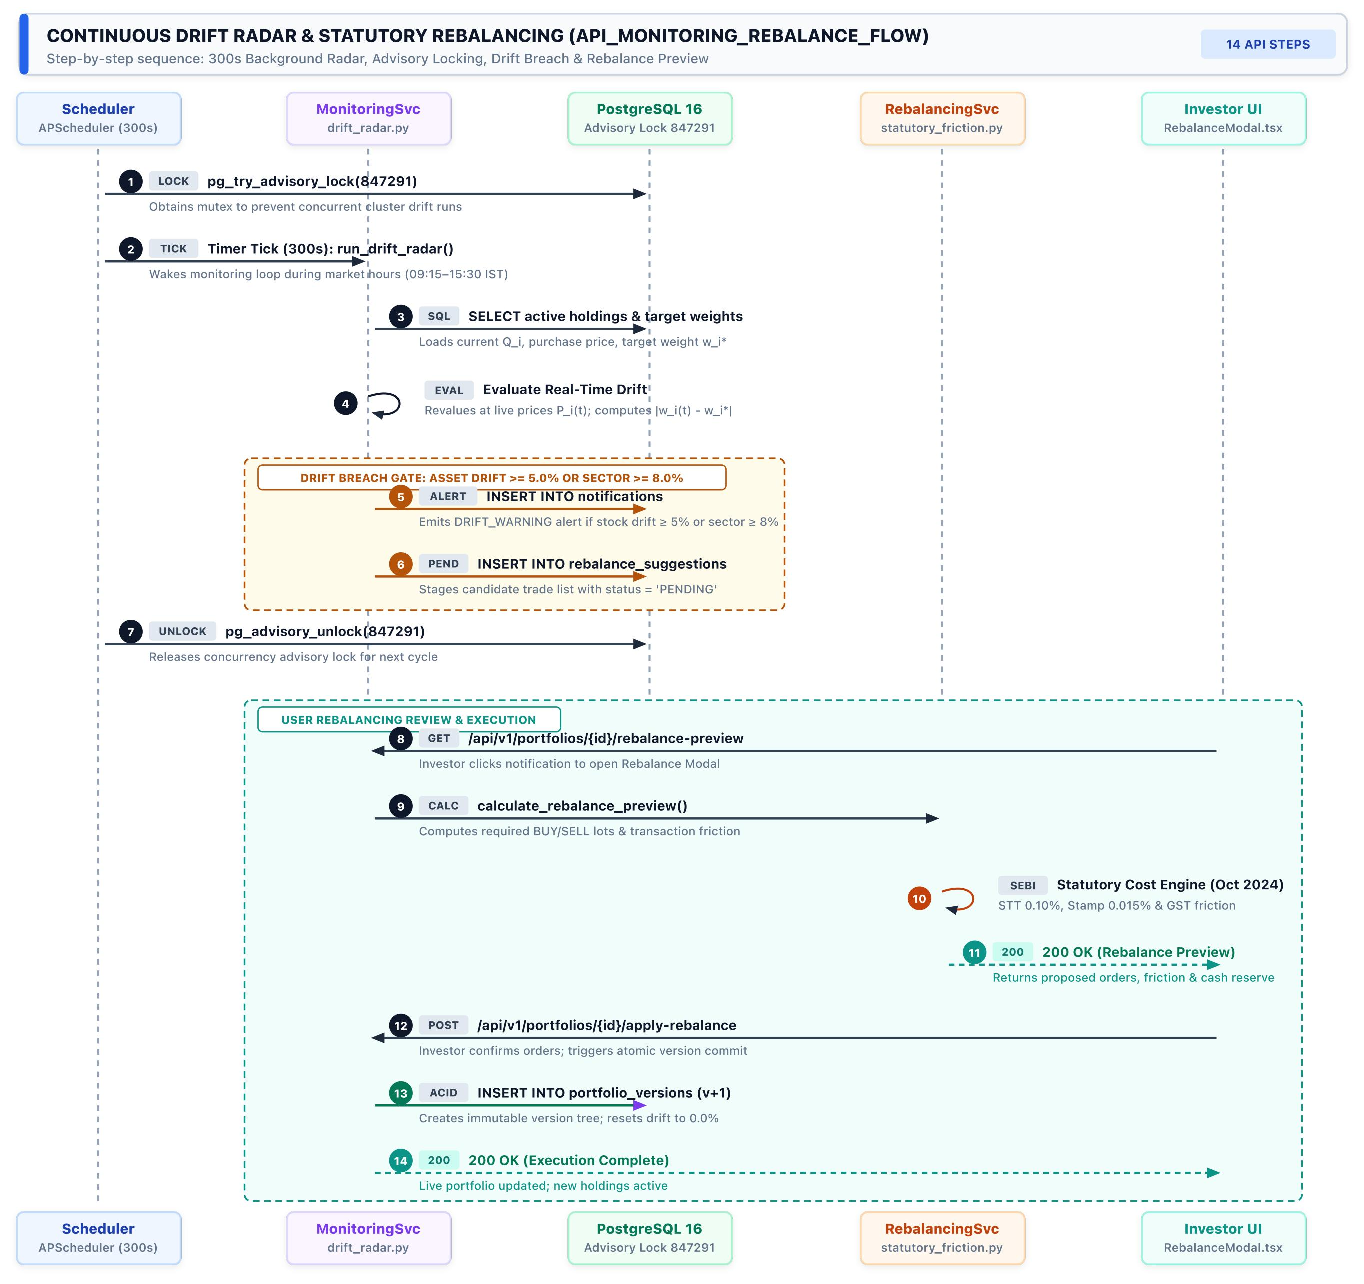
\includegraphics[width=\textwidth, height=0.72\textheight, keepaspectratio]{API_MONITORING_REBALANCE_FLOW.pdf}
    \caption{API Sequence Diagram: Continuous Drift Radar and Rebalance Preview Flow}
    \label{fig:api_mon_seq}
\end{figure}

\clearpage
\begin{figure}[p]
    \centering
    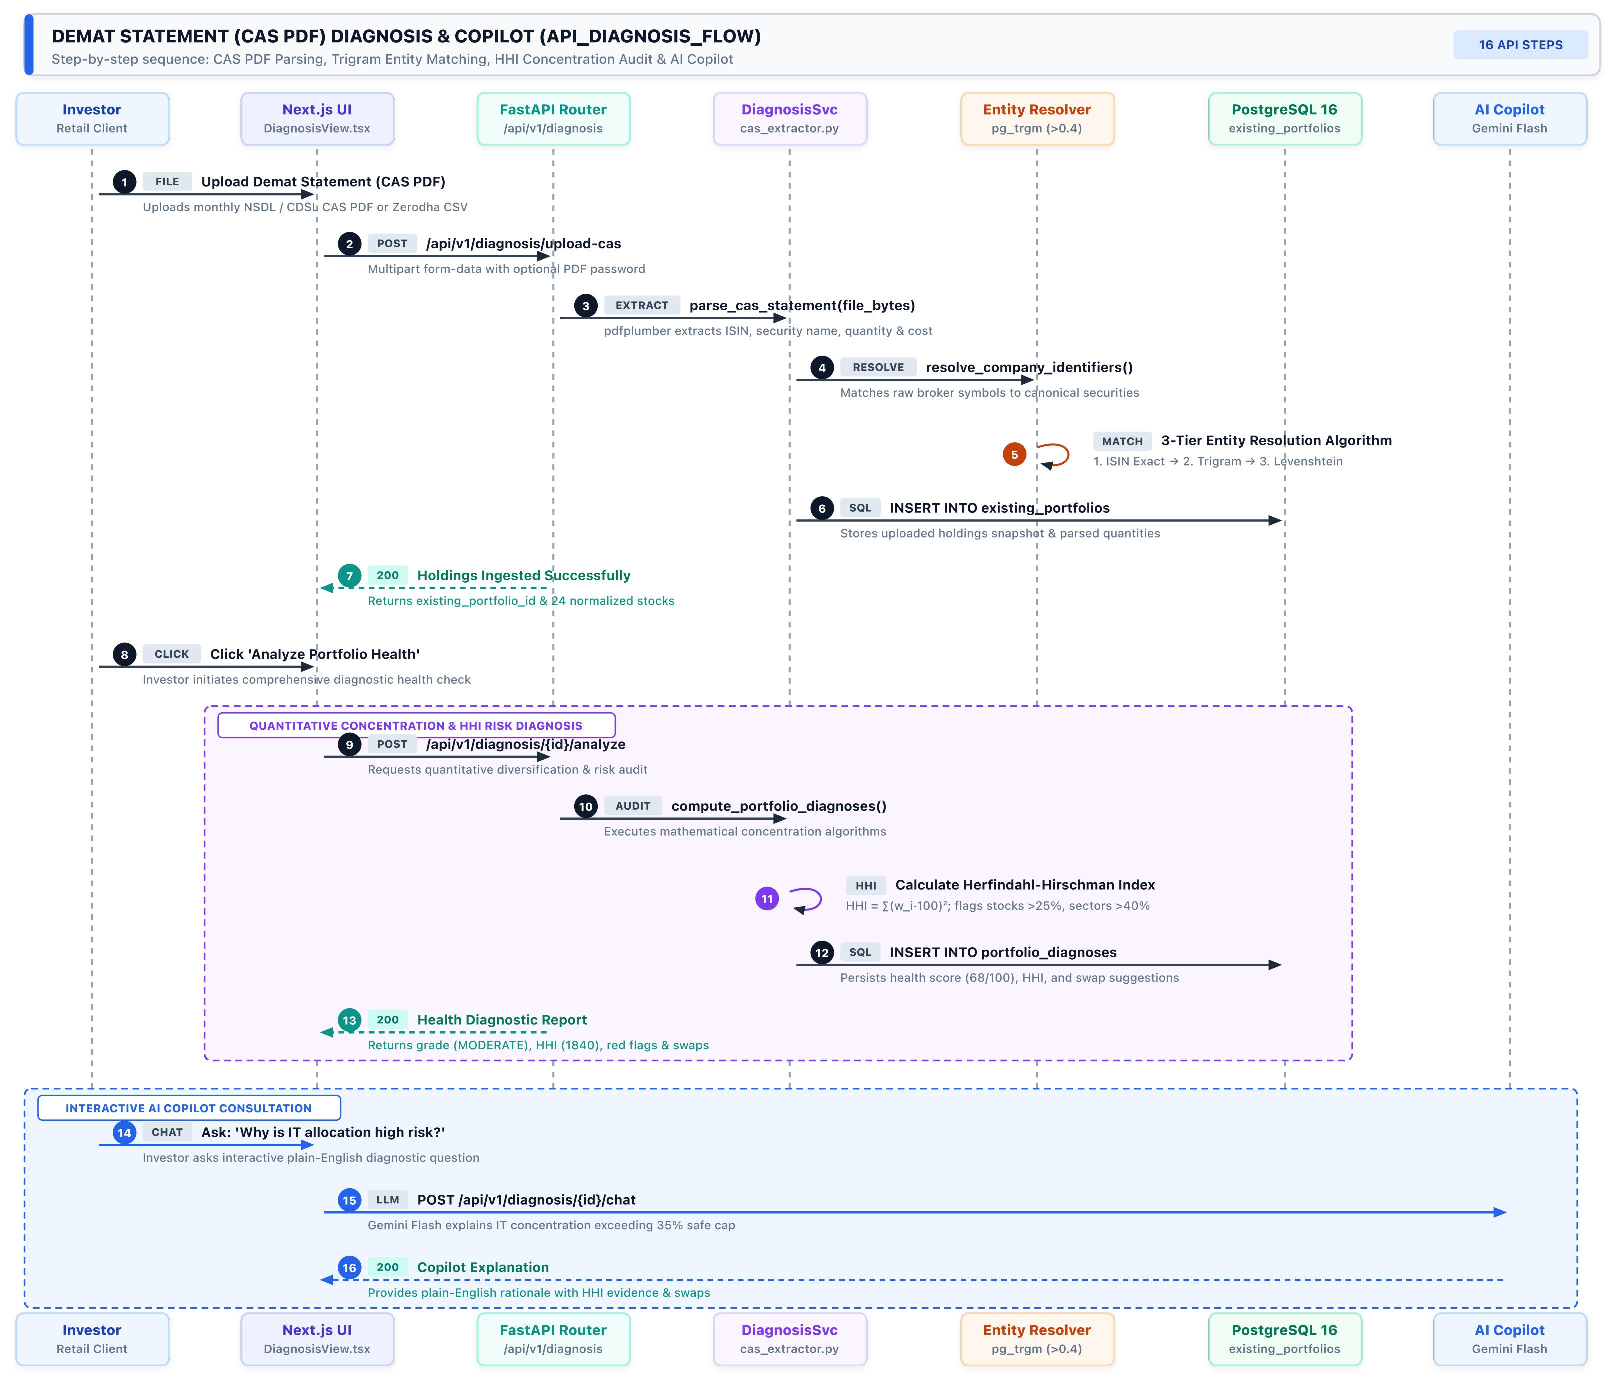
\includegraphics[width=\textwidth, height=0.72\textheight, keepaspectratio]{API_DIAGNOSIS_FLOW.pdf}
    \caption{API Sequence Diagram: Demat CAS Statement PDF Diagnosis Flow}
    \label{fig:api_diag_seq}
\end{figure}
\clearpage

\section{Postman Collection and Developer Testing Tools}
To allow engineers and system auditors to test the API easily, Lucid provides an importable Postman collection located in \texttt{postman/}:
\begin{itemize}
    \item \textbf{Collection File (\path{Lucid_API_Collection.json})}: Contains \textbf{96 API requests} organized across 16 folders covering all features.
    \item \textbf{Environment File (\path{Lucid_Development_Environment.json})}: Configured with server URLs and test developer credentials.
    \item \textbf{Automated Test Scripts}: When a developer runs the login request, Postman automatically captures the new session token and saves it into the active environment. All subsequent requests use this token automatically, enabling one-click test runs across the entire platform.
\end{itemize}
